%!TEX TS-program = xelatex
%!TEX encoding = UTF-8 Unicode

\documentclass[11pt,a4paper,oneside]{book}
\usepackage[margin=2.5cm]{geometry}

% ------------------------------------------------------------------------------
% customize the headers with fancyhdr package
% ------------------------------------------------------------------------------
\usepackage{fancyhdr}
\fancyhf{}
\fancyhead[LE]{\leftmark}
\fancyhead[RO]{\nouppercase{\rightmark}}
\fancyfoot[LE,RO]{\thepage}
\pagestyle{fancy}

% ------------------------------------------------------------------------------
% Index
% ------------------------------------------------------------------------------
\usepackage{makeidx}
\makeindex

% ------------------------------------------------------------------------------
% Hyperlinks
% ------------------------------------------------------------------------------
\usepackage[colorlinks=true,linkcolor=blue]{hyperref}
\usepackage[all]{hypcap}  % Be sure to call this package after loading hyperref.

% ------------------------------------------------------------------------------
% Glossaries, must be after hyperref
% ------------------------------------------------------------------------------
\usepackage[xindy,toc]{glossaries}
\makeglossaries{}

% ------------------------------------------------------------------------------
% load tocbibind to add contents,list of figures, list of tables and
% bibliography into the toc
% ------------------------------------------------------------------------------
% \usepackage[utf8]{inputenc}
% \usepackage[english]{babel}
\usepackage[
	backend=bibtex,
	natbib,
	style=authoryear,
	citestyle=authoryear,
	maxbibnames=99,
	maxcitenames=1
]{biblatex}
\addbibresource{dlbook-complete.bib}

% make the 'et al.' italic
\DefineBibliographyStrings{english}{%
    andothers = {\it et\addabbrvspace al\adddot}
}

% A workaround to fix a known bug in biblatex, see http://tex.stackexchange.com/questions/311426/bibliography-error-use-of-blxbblverbaddi-doesnt-match-its-definition-ve
\makeatletter
\def\blx@maxline{77}
\makeatother

% \usepackage{natbib}
\usepackage{tocbibind}

% ------------------------------------------------------------------------------
% Needed to level up the bibliography in the toc
% ------------------------------------------------------------------------------
\usepackage{bookmark}

\usepackage[figurename=图.]{caption}

% ------------------------------------------------------------------------------
% Needed to load images
% ------------------------------------------------------------------------------
\usepackage{graphicx}
\graphicspath{{./figures/}}   % where to look for images

% ------------------------------------------------------------------------------
% for long and nice table
% ------------------------------------------------------------------------------
\usepackage{longtable}
\usepackage{booktabs}
\usepackage{ltxtable}

% for compact item list
\usepackage{paralist}
% \usepackage{enumitem}
\usepackage[inline]{enumitem}
% for algorithm
\usepackage[chapter]{algorithm}
\usepackage{algorithmic}
% \usepackage{algpseudocode}

% \renewcommand{\thealgorithm}{\arabic{chapter}.\arabic{algorithm}} 

% ------------------------------------------------------------------------------
% Math - Warning: before cjkfonts (xeCJK) and other package loads fontspec
% ------------------------------------------------------------------------------
\usepackage{amsmath}
\usepackage{amsfonts}
\usepackage{amssymb}
\numberwithin{equation}{chapter}

% font selection for mathematics with XeLaTeX, MUST after amsfonts
\usepackage{mathspec}
% \setmathsfont(Digits,Latin,Greek)[Numbers={Lining,Proportional}]{Minion Pro}

% There's no italic sans-serif math font by default, but it's needed in this book
% follow: http://tex.stackexchange.com/questions/77640/bold-italic-and-sans-serif-math-symbols
% to define a \mathsfit{} macro
\DeclareMathAlphabet{\mathsfit}{\encodingdefault}{\sfdefault}{m}{sl}
\SetMathAlphabet{\mathsfit}{bold}{\encodingdefault}{\sfdefault}{bx}{sl}

% ------------------------------------------------------------------------------
% Tikz
% ------------------------------------------------------------------------------

\usepackage{tikz}
\usetikzlibrary{calc,positioning,arrows.meta,shapes.geometric,shapes.misc }

% ------------------------------------------------------------------------------
% Localization setting
% ------------------------------------------------------------------------------

% load cjkfonts package and set Noto Sans SC as the default CJK fonts:
\usepackage[default,mdseries=Light,bfseries=Medium]{cjkfonts}

\usepackage{titlesec}

\titleformat{\part}[display]
{\centering\bfseries\Huge}%
{\Huge 第 \thepart{} 部分}%
{12 pt}%
{\bfseries\Huge}%

\titleformat{\chapter}[display]
  {\bfseries\huge}%
  {\huge 第 \thechapter{} 章}%
  {10 pt}%
  {\bfseries\huge}%

\renewcommand{\contentsname}{目录}
\renewcommand{\indexname}{索引}
\renewcommand{\figurename}{图}
\renewcommand{\tablename}{表}

% Redefine \emph to be both bold and italic, better in chinese document
%\let\emph\relax
%\DeclareTextFontCommand{\emph}{\bfseries\em} % bold and italic
%\DeclareTextFontCommand{\emph}{\bfseries} % just bold

\usepackage{indentfirst}

% ------------------------------------------------------------------------------
% Western fonts setting
% ------------------------------------------------------------------------------

% Set Roboto and Source Code Pro, which are installed with TexLive, for western
% fonts:

% \usepackage[no-math]{fontspec}

\newcommand{\robotodir}[0]{fonts/}
\newcommand{\sourcecodeprodir}[0]{fonts/}
\newcommand{\sourceserifprodir}[0]{fonts/}

\newcommand{\robotomd}[0]{Light}
\newcommand{\robotobf}[0]{Medium}
\newcommand{\robotoit}[0]{LightItalic}
\newcommand{\robotobi}[0]{MediumItalic}
\newcommand{\codepromd}[0]{Light}
\newcommand{\codeprobf}[0]{Medium}
\newcommand{\codeproit}[0]{LightIt}
\newcommand{\codeprobi}[0]{MediumIt}
\newcommand{\serifpromd}[0]{Light}
\newcommand{\serifprobf}[0]{Semibold}

\newfontfamily\Roboto{Roboto}[
  Extension=.ttf,
  Path=\robotodir,
  UprightFont=*-Regular,
  BoldFont=*-Bold,
  ItalicFont=*-Italic,
  BoldItalicFont=*-BoldItalic]

\newfontfamily\SourceCodePro{SourceCodePro}[
  Extension=.otf,
  Path=\sourcecodeprodir,
  UprightFont=*-\codepromd,
  BoldFont=*-\codeprobf,
  ItalicFont=*-\codeproit,
  BoldItalicFont=*-\codeprobi]

\newfontfamily\SourceSerifPro{SourceSerifPro}[
  Extension=.otf,
  Path=\sourceserifprodir,
  UprightFont=*-\serifpromd,
  BoldFont=*-\serifprobf]

\newcommand{\serif}[0]{\SourceSerifPro}

\newfontfamily\RobotoThin{Roboto}[
  Extension=.ttf,
  Path=\robotodir,
  UprightFont=*-Thin,
  ItalicFont=*-ThinItalic]

\newfontfamily\RobotoLight{Roboto}[
  Extension=.ttf,
  Path=\robotodir,
  UprightFont=*-Light,
  ItalicFont=*-LightItalic]

\newfontfamily\RobotoRegular{Roboto}[
  Extension=.ttf,
  Path=\robotodir,
  UprightFont=*-Regular,
  ItalicFont=*-Italic]

\newfontfamily\RobotoMedium{Roboto}[
  Extension=.ttf,
  Path=\robotodir,
  UprightFont=*-Medium,
  ItalicFont=*-MediumItalic]

\newfontfamily\RobotoBold{Roboto}[
  Extension=.ttf,
  Path=\robotodir,
  UprightFont=*-Bold,
  ItalicFont=*-BoldItalic]

\newfontfamily\RobotoBlack{Roboto}[
  Extension=.ttf,
  Path=\robotodir,
  UprightFont=*-Black,
  ItalicFont=*-BlackItalic]
  
\setmainfont{Roboto}[
  Extension=.ttf,
  Path=\robotodir,
  UprightFont=*-\robotomd,
  BoldFont=*-\robotobf,
  ItalicFont=*-\robotoit,
  BoldItalicFont=*-\robotobi]

\setsansfont{Roboto}[
  Extension=.ttf,
  Path=\robotodir,
  UprightFont=*-\robotomd,
  BoldFont=*-\robotobf,
  ItalicFont=*-\robotoit,
  BoldItalicFont=*-\robotobi]

\setmonofont{SourceCodePro}[
  Extension=.otf,
  Path=\sourcecodeprodir,
  UprightFont=*-\codepromd,
  BoldFont=*-\codeprobf,
  ItalicFont=*-\codeproit,
  BoldItalicFont=*-\codeprobi]

% ------------------------------------------------------------------------------
% Line space
% ------------------------------------------------------------------------------
\usepackage{setspace}
\onehalfspacing{}

% ------------------------------------------------------------------------------
% Load glossaries
% ------------------------------------------------------------------------------
%% glossaries

%% Chapter 1

\newglossaryentry{ai}{
  name={人工智能},
  description={\emph{Artifical Intelligence}, AI}
}

\newglossaryentry{dl}{
  name={深度学习},
  description={\emph{Deep Learning}}
}

\newglossaryentry{knowledge-base}{
  name={知识库},
  description={\emph{Knowledge Base}}
}

\newglossaryentry{ml}{
  name={机器学习},
  description={\emph{Machine Learning}}
}

\newglossaryentry{logistic-regression}{
  name={逻辑回归},
  description={\emph{Logistic Regression}}
}

\newglossaryentry{representations}{
  name={表征},
  description={\emph{Representations},表征是信息的呈现方式}
}

\newglossaryentry{rep-learning}{
  name={表征学习},
  description={\emph{Representation Learning}}
}

\newglossaryentry{autoencoder}{
  name={自动编码器},
  description={\emph{Autoencoder (s)}}
}

\newglossaryentry{encoder}{
  name={编码器},
  description={\emph{encoder}}
}

\newglossaryentry{decoder}{
  name={解码器},
  description={\emph{decoder}}
}

%% Chapter 12

\newglossaryentry{weight}{
  name={权重},
  description={\emph{Weight}}
}

\newglossaryentry{bias}{
  name={偏置},
  description={\emph{Bias}}
}

\newglossaryentry{SGD}{
  name=SGD,
  description={\emph{Stochastic Gradient Descent}, 随机梯度下降算法}
}

\newglossaryentry{warps}{
  name={线程束},
  description={\emph{Warps},同时运行的一组线程的称呼}
}

\newglossaryentry{overfitting}{
  name={过度拟合},
  description={\emph{overfitting},过度拟合,过拟合,过适}
}

\newglossaryentry{generalization_error}{
  name={泛化误差},
  description={\emph{Generalization error},泛化误差}
}

\newglossaryentry{dropout}{
  name={弃权},
  description={\emph{Dropout}, 弃权}
}

\newglossaryentry{bdt}{
  name={提高决策树},
  description={\emph{Boosted decision trees}}
}

\newglossaryentry{gcn}{
  name={全局对比度归一化},
  description={\emph{Global contrast normalization}, 全局对比度归一化}
}

\newglossaryentry{minibatch}{
  name={小批量},
  description={\emph{Minibatch}, 小批量}
}

% ------------------------------------------------------------------------------
% The document body
% ------------------------------------------------------------------------------

\begin{document}

% file: title.tex

\begin{titlepage}
\begin{center}
  \hfill\\
  \vspace{1cm}
  % title of this document
  {\fontsize{36pt}{40pt}\NotoSansSCBold{} 深度学习}\\
  \vspace{1em}
  {\LARGE\serif \href{http://www.deeplearningbook.org/}{Deep Learning}}\\
  \vspace{1cm}
  %\includegraphics{cayley}\\
  \vspace{1cm}
  
  {\large\serif
  \begin{tabular}{c}
    Ian Goodfellow \\
    Yoshua Bengio \\
    Aaron Courville
  \end{tabular}
  }
   
  \vfill
  {\large \today}\\
  \vspace{1em}
  {\large Draft}
\end{center}
\end{titlepage}


\frontmatter

%\maketitle

\tableofcontents
%\listoffigures
%\listoftables

\pagebreak

\chapter{致谢}
\label{ch:Acknowledgements}

没有许多人的贡献,本书是不可能完成的。

\chapter{数学符号}
\label{ch:notation}

这一部分提供了一个简明的索引,描述整本书中使用的数学符号。如果你不熟悉任何对应的
数学概念,这个符号索引可能看起来很吓人。然而,不要绝望,我们在 2 --- 4 章里描述了
这些概念的大部分。

\begin{center}
\setstretch{1.5}
{\Large\bfseries 数和数组}\\
\vspace{1em}
\begin{tabular}{c l}
  $a$ & 标量(整数或实数)\\
  $\pmb{a}$ & 向量 \\
  $\pmb{A}$ & 矩阵 \\
  $\mathsf{A}$ & 张量 \\
  $\pmb{I}_n$ & $n$ 行 $n$ 列的单位矩阵 \\
  $\pmb{I}$ & 单位矩阵,其维度隐含在上下文中 \\
  $\pmb{e}^{(i)}$ & 标准的基向量 $[0, \ldots, 0, 1, 0, \ldots, 0]$,$1$ 的位置由 $i$ 确定 \\
  $diag(\pmb{a})$ & 方块对角矩阵,其对角线元素为 $\pmb{a}$ \\
  $\mathrm{a}$ & 标量随机变量 \\
  $\mathbf{a}$ & 向量值随机变量 \\
  $\mathbf{A}$ & 矩阵值随机变量
\end{tabular}
\end{center}

\vspace{1em}

\begin{center}
\setstretch{1.5}
{\Large\bfseries 集合和图}\\
\vspace{1em}
\begin{tabular}{c l}
  $\mathbb{A}$ & 集合 \\
  $\mathbb{R}$ & 实数集合 \\
  ${0,1}$ & 包含 $0$ 和 $1$ 的集合 \\
  ${0,1,\ldots,n}$ & $0$ 到 $n$ 的所有整数集合 \\
  $[a,b]$ & 包括 $a$ 和 $b$ 的实数区间 \\
  $(a,b]$ & 左开右闭区间,不包括 $a$ 但包括 $b$ \\
  $\mathbb{A}\backslash\mathbb{B}$ & 集合差,例如,包含有 $\mathbb{A}$ 的元素但其不在 $\mathbb{B}$ 中的集合 \\
  $\mathcal{G}$ & 图 \\
  $Pa_{\mathcal{G}}(x_i)$ & 图  $\mathcal{G}$ 中 $x_i$ 的父顶点
\end{tabular}
\end{center}

\vspace{1em}

\begin{center}
\setstretch{1.5}
{\Large\bfseries 索引}\\
\vspace{1em}
\begin{tabular}{c l}
  $a_i$ & 向量 $\pmb{a}$ 的第 $i$ 个元素,索引起始位置为 $1$ \\
  $a_{-i}$ & 除了第 $i$ 个元素的向量 $\pmb{a}$ 的所有元素 \\
  $A_{i,j}$ & 矩阵 $\pmb{A}$ 的 $i,j$ 位置元素
\end{tabular}
\end{center}


\mainmatter{}

% intro.tex

\chapter{介绍}
\label{ch:intro}

长久以来,发明家们梦想着创造会思考的机器。这种愿望至少可以追溯到古希腊时代。神话
人物皮格马利翁,代达罗斯和赫菲斯托斯都可以被理解为传说中的发明家,而伽拉泰亚,塔
罗斯和潘多拉都可以被看作是人工生
命\citep{ovid2004metamorphoses,sparkes1996red,1997works}。

当可编程计算机最初被设想时~——~在它被建造的超过一百年前~——~人们就想知道它们是否可
能变得智能\citep{Lovelace1842}。今天,\emph{\gls{ai} (AI)} 是一个茁壮成长的领域,
有着许多实际应用和活跃的研究课题。我们期待智能软件来自动化日常的劳动,理解语音或
图像,进行医学诊断和支持基础科学研究。

在\gls*{ai}早期,这个领域快速处理和解决一些问题,这些问题在脑力上对人类来说困难但
对计算机来说则相对直接~——~这些问题可以通过一份有条理的、数学规则的列表形式来描
述。\gls*{ai}的真正的挑战是解决那些容易被人执行,但是难于规范描述的任务~——~那些我
们凭直觉不假思索就能解决的问题,例如识别语音中的单词或者图像中的人脸。

这本书是关于这些更直观的问题的一个解决方案。这个解决方案是让计算机从经验中学习,
并以概念层次的形式理解这个世界,其中的每一个概念以和它相联系的更简单的概念形式定
义。通过从经验中收集知识,这种方法避免了需要人类操作者规范地去指定计算机需要的所
有知识。概念的层次结构允许计算机通过建立更简单的概念来学习复杂的概念。如果我们绘
制一个图,显示这些概念是如何建立在彼此之上的,这幅图会很深,有许多层。因为这个原
因,我们称这种人工智能的方法为\emph{\gls{dl}}。

许多早期的成功的人工智能发生在相对毫无新意和规范的环境中,并没有需要电脑有太多的
对世界的理解。例如,IBM 的深蓝对弈系统在 1997 年击败了世界冠军卡斯帕罗
夫\citep{Hsu2002}。国际象棋是一个很简单的世界,只包含 64 个位置和 32 个移动方式受
到严格限制的棋子。设计一个成功的国际象棋战略是一个巨大的成就,但是因为描述棋子的
集合和移动的困难性,这对计算机不算是挑战。象棋能够通过一个非常简短的完整规则的列
表来完整描述,很容易由程序员提前提供。

具有讽刺意味的是,对一个人类的来说最困难的脑力工作中那些抽象和规范的任务,对计算
机则是最简单的。计算机很早就能够击败即使是最优秀的人类国际象棋选手,但最近才能与
一般人的能力相匹配地识别物体或语音。一个人的日常生活需要大量的关于世界的知识。很
多这方面的知识是主观的和直观的,因此很难以一种规范的方式表达。计算机需要捕捉到相
同的知识,以便表现为一种智能的方式。人工智能中的一个关键的挑战是如何将这些非规范
的知识转化进计算机。

几个\gls*{ai}项目寻求用规范的语言来硬编码对于世界的理解。一台计算机可以自动使用逻
辑推理规则来对这些规范语言中的语句进行推理。这被称为人工智能
的\emph{\gls{knowledge-base}}\,方法。这些项目没有一个导致重大的成功。其中一个最著
名的项目是 Cyc\citep{Lenat-1989-book}。Cyc 是一个推理引擎和以一种称为 CycL 语言形
式的语句数据库。这些语句是由一个人类监督者输入的。这是一个笨拙的过程。人们费很大
劲来设计有条理的规则,这些规则具有足够的复杂性来准确描述这个世界。例如,Cyc 未能
理解一个关于一个名叫 Fred 的人在早晨刮脸的故事\citep{MachineChangedWorld}。它的推
理引擎检测到故事中前后矛盾的地方:它知道人类没有电子器件,但是因为 Fred 正好拿着
一个电子剃须刀,它坚信这个 ``正在刮脸的 Fred'' 包含有电子器件。于是它询问当 Fred
在刮脸时还是不是一个人类。

依赖于硬编码知识的系统面对的困难,表明 AI 系统需要获得它们自己知识的能力~——~通过
从原始数据中提取模式的能力。这个能力被称为\emph{\gls{ml}}。\gls*{ml}的引入允许计
算机处理涉及到真实世界的问题,并且做出显得主观的决定。一个简单的被称
为\emph{\gls{logistic-regression}}\,的\gls*{ml}算法能够确定是否建议剖腹
产\citep{MorYosef90}。另一个简单的被称为 \emph{naive Bayes} 的\gls*{ml}算法,能够
从垃圾邮件中区分出合理的邮件。

这些简单的\gls*{ml}算法的性能重度依赖给予它们的数据
的\emph{\gls{representations}}。例如,当\gls*{logistic-regression}被用在建议剖腹
产时,AI 系统不直接检查病人。相反,医生告诉这个系统一些相关信息,例如有没有子宫疤
痕。每段包含在病人描述中的信息被称为\emph{特征}。\gls*{logistic-regression}学习病
人的每个特征如何与不同的结果想关联。然而,它不能对任意方式定义的特征起作用。如果
给\gls*{logistic-regression}一幅病人的 MRI 扫描,而不是医生格式化后的报告,它无法
做出有用的预测。MRI 扫描中独特的像素和分娩中可能发生的并发症有负面的相关性。

这种对\gls*{representations}的依赖是一个普遍的现象,出现在整个计算机科学,甚至日
常生活中。在计算机科学中,诸如搜索一个数据的集合这样的操作,如果这个集合被很好地
结构化和智能地索引,那么这个搜索可以以指数级别加快处理,人们可以很容易地在阿拉伯
数字上执行算术运算,但在罗马数字做算术更为耗时。这是不足为奇的,
对\gls*{representations}的选择在\gls*{ml}算法的性能上有巨大的影响。一个简单的可视
化示例,参见图~\ref{fig:different_representations}。

\begin{figure}[h]
  \centering
  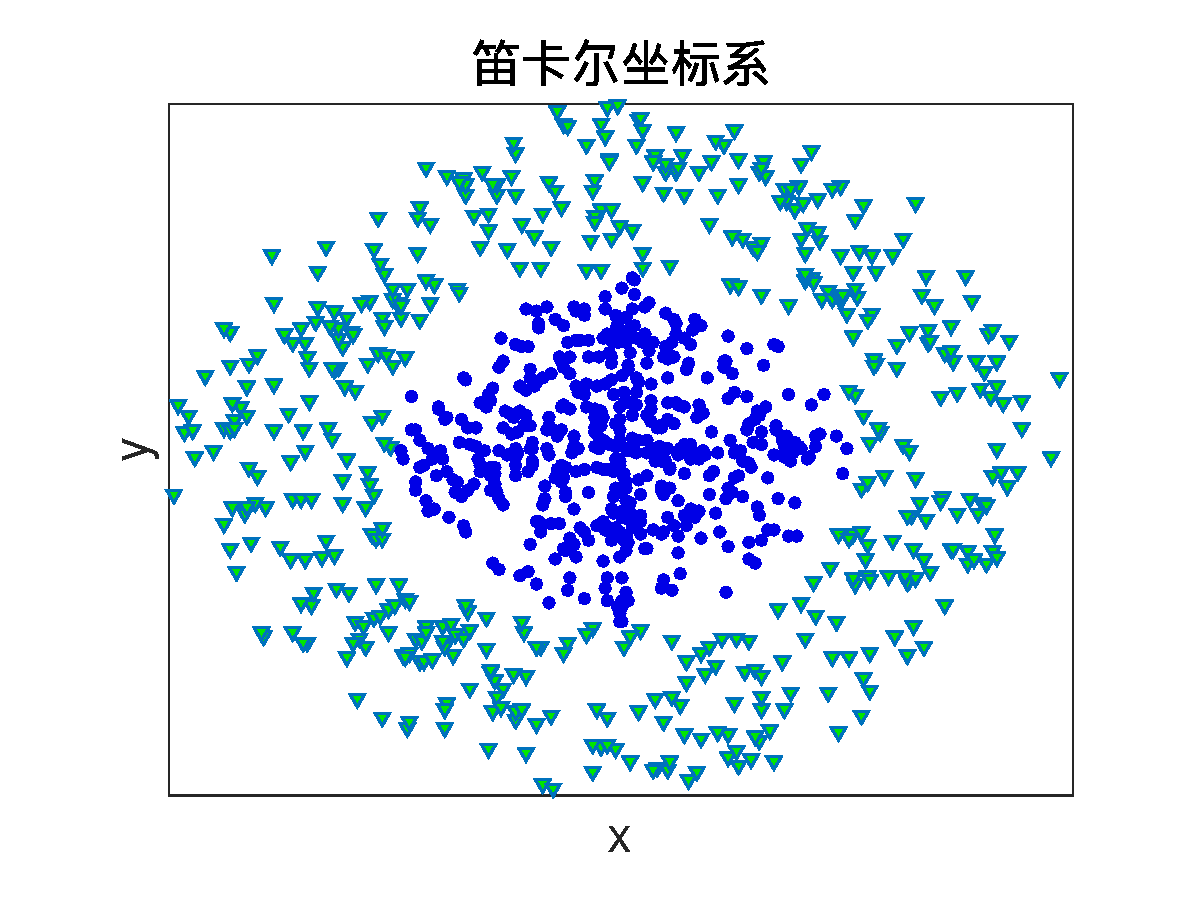
\includegraphics[width=0.45\textwidth]{cartesian_scatter}
  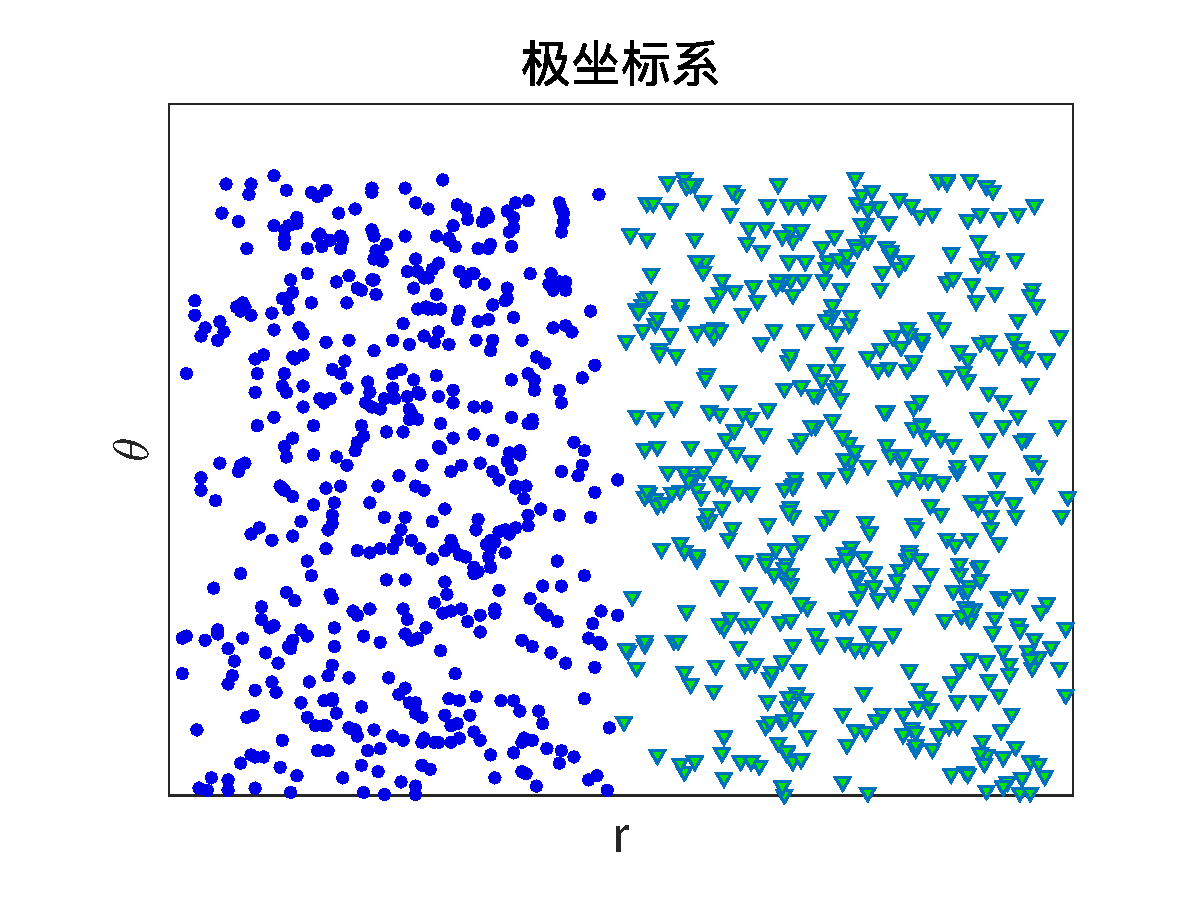
\includegraphics[width=0.45\textwidth]{polar_scatter}
  \caption{不同\gls*{representations}的例子:假设我们想要在一幅散点图中画一条线来
    区分两种数据。在左边的图中,我们使用笛卡尔坐标系描述一些数据,而这个任务是不
    可能的。在右边的图中,我们用极坐标描述一些数据,这个任务就变得很容易用一条竖
    线来解决。这个图由 David Warde-Farley 协助生
    成。\label{fig:different_representations}}
\end{figure}

这个问题的一个解决方法是使用\gls*{ml}来探索不只是从\gls*{representations}到输出的
映射,还有\gls*{representations}本身。这个方法被称为\emph{\gls{rep-learning}}。学
习过的\gls*{representations}往往会导致比手工设计的\gls*{representations}更好的性
能。它们还允许 AI 系统以最少的人为干预来快速地适应新的任务。一
个\gls*{rep-learning}算法可以在几分钟内为一个简单的任务发现一个很好的特征集,或者
对一个复杂的任务,需要几个小时到几个月。手动为一个复杂的任务设计特征需要大量的时
间和人力;它可能耗费整个研究社区几十年的时间。

一个\gls*{rep-learning}算法的典型例子是\emph{\gls{autoencoder}}。一
个\gls*{autoencoder}由一个\emph{\gls{encoder}}\,和一个\emph{\gls{decoder}}\,组
成,\gls*{encoder}将输入数据转换为不同形式的表征,\gls*{decoder}将新的表征转换回
原始格式。\gls*{autoencoder}被训练成当一个输入进
过\gls*{encoder}然后\gls*{decoder}时保存尽可能多的信息,但也被训练使得新的表征有
各种很好的特性。不同种类的\gls*{autoencoder}的目的是获得不同性质的特性。

当为了学习特征而设计特征或算法时,我们的目标通常是分离能解释被观察数据
的\emph{\gls{fov}}。在这种背景下,我们用单词``因子''来简单指不同的影响来源;因子
通常不由乘法组合。

\section{谁应该读这本书?}

\section{深度学习的历史趋势}



\subsection{不断增长的模型规模}
\label{subsec:increasing_model_sizes}

% file: part_basics.tex
% source: http://www.deeplearningbook.org/contents/part_basics.html

\part{应用于本书的数学和机器学习基础}
\label{part_basics}

本书的这一部分介绍理解深度学习所需要的基本的数学概念。我们从应用于本书的数学的一
般概念开始,这些数学允许我们定义多元函数,找到这些函数的最高和最低点,并量化置信
度。

接下来,我们描述机器学习的基本目标。我们描述如何通过指定一个代表某些置信度的模型
来完成这些目标,设计一个衡量这些置信度与现实有多符合的代价函数,并用一个训练算法
来最小化那个代价函数。

这个基本框架是各种各样机器学习算法的基础,包括非深度机器学习的方法。在本书随后部
分中,我们在这个框架内开发深度学习算法。

\chapter{线性代数}
\label{ch:linear_algebra}

线性代数是广泛使用在整个科学和工程中的一个数学分支。然而,由于线性代数是一种连续
的形式而不是离散数学,许多计算机科学家对它少有经验。很好地理解线性代数,对理解和
使用许多\gls*{ml}算法来工作,是必不可少的,对\gls*{dl}尤其如此。因此,我们在介
绍\gls*{dl}之前先专注于对关键的线性代数必备知识做些陈述。

如果你已经熟悉了线性代数,尽管跳过这一章。如果你对这些概念有了一些先期的经验,但
是需要一个详细的参考来复习关键的公式,我们推荐 \emph{The Matrix Cookbook}
\citep{matrix-cookbook}。如果你完全没有接触过线性代数,这一章会教你足够的知识来阅
读本书,但是我们强烈建议你也去咨询其它专门教授线性代数的材料,例
如\citep{shilov1977linear}。本章会完全略过很多重要的线性代数的主题,它们对理
解\gls*{dl}不是必须的。

\section{标量、向量、矩阵和张量}
\label{scalars_vectors_matrices_and_tensors}

线性代数的研究涉及到几种数学对象的类型:

\begin{itemize}
\item \emph{\gls{scalars}}:一个标量仅仅是一个单独的数字,相反,大多数其它线性代
  数的研究对象通常是多个数组。我们用斜体来写标量。我们通常用小写命名标量。当我们
  介绍它们时,我们指定它们是什么样的数字。例如:当定义一个实数值的标量时,我们可
  能说``设 $s \in \mathbb{R}$ 为直线的斜率'',或者,当定义一个自然数标量
  时,``设 $n \in \mathbb{N}$ 为单元的个数''。
\item \emph{\gls{vecs}}:一个\gls*{vec}是一个数组。这些数字按照顺序排列。我们可以
  通过这一顺序中的索引来确定每一个单独的数字。通常我们以小写的粗体字体
  给\gls*{vec}命名,例如 $\pmb{x}$。\gls*{vec}的元素以伴有下标的斜体字体表
  示。$\pmb{x}$ 的第一个元素是 $x_1$,第二个是 $x_2$,依此类推。我们还要说
  明\gls*{vec}中存储的是什么类型的数字。如果每个元素是 $\mathbb{R}$ 中的数,
  而\gls*{vec}有 $n$ 个元素,那么\gls*{vec}位于以 $\mathbb{R}$ 的 $n$ 次笛卡尔积
  的所形成的集合内,表示为 $\mathbb{R}^n$。当我们需要显式地表示一个\gls*{vec}中的
  元素,我们把它们写成方括号围起来的一列:
  \begin{equation}
    x = \begin{bmatrix}x_1\\ x_2\\ \vdots\\ x_n\end{bmatrix}
    \label{eq:vec_example}
  \end{equation}
  我们可以把\gls*{vec}看做表示空间的点,每个元素提供沿着不同坐标轴的坐标。\\
  有时候我们需要索引一个向量中的一个元素集合。在这种情况下,我们定义一个包含索引
  的集合,并把这个集合写成一个下标。例如,为了获得 $x_1$,$x_3$ 和 $x_6$,我们定
  义集合 $S = {1, 3, 6}$,写为 $\pmb{x}_S$。我们使用 $-$ 标记表示一个集合的补充。
  例如 $\pmb{x}_{-1}$ 是包含 $\pmb{x}$ 中除了 $x_1$ 的所有元素
  的\gls*{vec},而 $\pmb{x}_{-S}$ 是包含 $\pmb{x}$ 中除了 $x_1$,$x_2$ 和 $x_6$
  之外的所有元素的向量。
\item \emph{\gls{matrices}}:一个矩阵是一个数字的二维数组,所以每个元素由两个索引
  确定,而不是一个。我们通常用大写的粗体字体表示矩阵,例如 $\pmb{A}$。如果一个实
  数值的矩阵 $\pmb{A}$ 高度为 $m$,宽度为
  $n$,那么我们说$\pmb{A} \in \mathbb{R}^{m \times n}$。我们通常使用斜体~——~但不
  是粗体字体~——~表示一个矩阵的元素,索引用逗号分开列出。例
  如,$A_{1,1}$ 是 $\pmb{A}$ 左上角的元素,而 $A_{m,n}$ 是右下角的元素。我们可以
  为横向坐标写一个 ``:'' 来表示所有竖向坐标 $i$ 的数字。例如,$\pmb{A}_{i,:}$ 表
  示竖向坐标 $i$ 的横跨 $\pmb{A}$ 的部分。即 $\pmb{A}$ 的第 $i$ 行。同样
  的,$\pmb{A}_{:,i}$ 是 $\pmb{A}$ 的第 $i$ 列。当我们需要显式地表示一个矩阵的元
  素,我们把它们写成一个用方括号围起来的数组:
  \begin{equation}
    \begin{bmatrix}A_{1,1} & A_{1,2} \\ A_{2,1} & A_{2,2}\end{bmatrix}
    \label{eq:matrix_example}
  \end{equation}
  有时候我们可能需要索引矩阵值的表达式,它不仅仅是一个单个的字母。在这种情况下,
  我们在表达式后使用下标,但不转换为小写。例如,$f(\pmb{A})_{i,j}$ 给出了应用函
  数 $f$ 到 $\pmb{A}$ 上后计算得到的 $(i,j)$ 位置的元素。。
\item \emph{\gls{tensors}}:在有些情况下我们会需要一个多于两个坐标的数组。在一般
  情况下,排列在一个规则的网格~——~具有可变数量的坐标轴~——~上的数组,被称为一
  个\emph{\gls{tensor}}。我们用这样的字体表示一个名为 ``A'' 的张
  量:$\pmb{\mathsf{A}}$。我们把表示 $\pmb{\mathsf{A}}$ 在 $(i,j,k)$ 坐标的元素写
  为 $\mathsfit{A}_{i,j,k}$。
\end{itemize}

矩阵的一个重要的操作是\emph{\gls{transpose}}。一个矩阵的\gls*{transpose}是将矩阵
沿着一个对角线~——~称为\emph{\gls{main-diag}},从左上角指向右下角~——~做镜像。参见
图~\ref{fig:transpose_of_matrix} 中对这个操作的图形化描述。我们把一个矩
阵 $\pmb{A}$ 的转置表示为 $\pmb{A}^{\top}$,以这样定义
\begin{equation}
  (\pmb{A}^{\top})_{i,j} = A_{j,i}
  \label{eq:transpose_of_matrix}
\end{equation}

\begin{figure}[h]
  \centering
  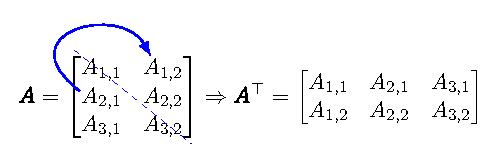
\includegraphics{transpose_of_matrix}
  \caption{矩阵的转置可以被看做沿着\gls*{main-diag}的镜
    像\label{fig:transpose_of_matrix}}
\end{figure}

\gls*{vecs}可以被看做是只含有一列的矩阵。如此一个\gls*{vec}的\gls*{transpose}就是
一个只有一行的矩阵。有时候这样定义一个\gls*{vec}:在一行的矩阵的文本区中写出它的
元素,然后使用一个\gls*{transpose}操作来把它转换成标准的列\gls*{vec},例
如,$\pmb{x} = [x_1, x_2, x_3]^{\top}$。

一个标量可以被看做是只有一个元素的矩阵。因此,我们可以看到一个标量就是它自己
的\gls*{transpose}:$a = a^{\top}$。

只要矩阵有相同的形状,我们可以把它们相互相加,只需要将它们对应的元素相
加:$\pmb{C} = \pmb{A} + \pmb{B}$,这里 $C_{i,j} = A_{i,j} + B_{i,j}$。

我们也可以把一个标量加到一个矩阵上,或者用一个标量乘以一个矩阵,只需要在矩阵上执
行操作:$\pmb{D} = a \cdot \pmb{B} + c$,这里 $D_{i,j} = a \cdot B_{i,j} + c$。

在\gls*{dl}的环境中,我们也使用一些较传统的符号。我们允许矩阵和一个\gls*{vec}相加,
产生另一个矩阵:$\pmb{C} = \pmb{A} + \pmb{b}$,这里
$C_{i,j} = A_{i,j} + b_j$。换句话说,\gls*{vec} $\pmb{b}$ 被加到矩阵的每一行。这
个速记法消除了需要在相加前定义一个复制 $\pmb{b}$ 到每一行的矩阵。这个 $\pmb{b}$
到多个位置的隐式拷贝被称为\emph{\gls{broadcasting}}。

\section{矩阵和向量的乘法}
\label{sec:multiplying_matrices_and_vectors}

涉及矩阵的最重要的操作之一是两个矩阵的乘法。矩
阵 $\pmb{A}$ 和 $\pmb{B}$ 的\emph{\gls{matrix-product}}\,是另一个矩阵
$\pmb{C}$。为了这种积可定义,$\pmb{A}$ 的列数量必须和 $\pmb{B}$ 的行数相同。如
果 $\pmb{A}$ 的形状为 $m \times n$,而 $\pmb{B}$ 的形状为 $n \times p$,那
么 $\pmb{C}$ 的形状为 $m \times p$。我们可以把两个或更多矩阵放在一起来
写\gls*{matrix-product},例如:
\begin{equation}
  \pmb{C} = \pmb{A}\pmb{B}
  \label{eq:matrix_product}
\end{equation}

乘积操作被定义为:
\begin{equation}
  C_{i,j} = \sum_{k}A_{i,k}B_{k,j}
  \label{eq:product_operation}
\end{equation}

注意两个矩阵的标准乘积\textbf{不}仅仅是一个包含有单独元素乘积的矩阵。这样的操作是
存在的,并被称为\emph{\gls{element-product}}\,或者\emph{\gls{hadamard-product}},
表示为 $\pmb{A} \odot \pmb{B}$。

两个具有相同维度的\gls*{vecs}
$\pmb{x}$ 和 $\pmb{y}$ 的\emph{\gls{dot-product}}\,是\gls*{matrix-product}
$\pmb{x}^{\top}\pmb{y}$。我们可以把\gls*{matrix-product} $\pmb{C} =
\pmb{A}\pmb{B}$ 看做计
算 $\pmb{A}$ 的第 $i$ 行和 $\pmb{B}$ 的第 $j$ 列的\gls*{dot-product} $C_{i,j}$。

\gls*{matrix-product}操作有很多有用的特性,使得对矩阵的数学分析更方便。例如,矩阵
的乘法是可分配的:
\begin{equation}
  \pmb{A}(\pmb{B} + \pmb{C}) = \pmb{A}\pmb{B} + \pmb{A}\pmb{C}
  \label{eq:distributive_matrix_multiplication}
\end{equation}
也可结合:
\begin{equation}
  \pmb{A}(\pmb{B}\pmb{C}) = (\pmb{A}\pmb{B})\pmb{C}
  \label{eq:associative_matrix_multiplication}
\end{equation}
不像标量乘法,矩阵乘法是\textbf{不}可交换的($\pmb{A}\pmb{B} = \pmb{B}\pmb{A}$ 的
条件并不总是成立)。但是,两个\gls*{vecs}之间的\gls*{dot-product}是可交换的:
\begin{equation}
  \pmb{x}^{\top}\pmb{y} = \pmb{y}^{\top}\pmb{x}
  \label{eq:commutative_vec_multiplication}
\end{equation}

\gls*{matrix-product}的\gls*{transpose}有一个简单的形式:
\begin{equation}
  (\pmb{A}\pmb{B})^{\top} = \pmb{B}^{\top}\pmb{A}^{\top}
  \label{eq:transpose_of_matrix_product}
\end{equation}

这使我们利用这样一个乘积值为一个标量时,它和自己的\gls*{transpose}相等的事实,来
证明方程~\ref{eq:commutative_vec_multiplication}:
\begin{equation}
  \pmb{x}^{\top}\pmb{y} = (\pmb{x}^{\top}\pmb{y})^{\top} = \pmb{y}^{\top}\pmb{x}
  \label{eq:demonstrate_commutative_vec_multiplication}
\end{equation}

由于这本教科书的重点不是线性代数,我们在这里不会试图列出全面
的\gls*{matrix-product}的有用特性,但读者应该知道有更多。

现在我们知道了足够的线性代数的数学符号来写下一个线性方程的系统:
\begin{equation}
  \pmb{A}\pmb{x} = \pmb{b}
  \label{eq:system_of_linear_equations}
\end{equation}
这里 $\pmb{A} \in \mathbb{R}^{m \times n}$ 是一个已知的矩阵,$\pmb{b} \in
\mathbb{R}^m$ 是一个已知的\gls*{vec},而 $\pmb{x} \in \mathbb{R}^n$ 是一个我们想
要解出的未知变量的\gls*{vec}。$\pmb{A}$ 的每一行和 $\pmb{b}$ 的每个元素提供了另一
个限制。我们可以重写方程~\ref{eq:system_of_linear_equations} 为:
\begin{align}
  \pmb{A}_{1,:}\pmb{x} &= b_1\\
  \pmb{A}_{2,:}\pmb{x} &= b_2\\
  \ldots \\
  \pmb{A}_{m,:}\pmb{x} &= b_m
\end{align}

或者,甚至更明确地:
\begin{align}
  \pmb{A}_{1,1}x_1 + \pmb{A}_{1,2}x_2 + \ldots + \pmb{A}_{1,n}x_n = b_1 \\
  \pmb{A}_{2,1}x_1 + \pmb{A}_{2,2}x_2 + \ldots + \pmb{A}_{2,n}x_n = b_2 \\
  \ldots \hspace{7em} \\
  \pmb{A}_{m,1}x_1 + \pmb{A}_{m,2}x_2 + \ldots + \pmb{A}_{m,n}x_n = b_m
\end{align}

矩阵--\gls*{vec}乘积的符号提供了这种方程形式的一个更紧凑的表示。

\section{单位矩阵和逆矩阵}
\label{sec:identity_and_inverse_matrices}

线性代数提供一个强大的工具,被称为\emph{\gls{matrix-inversion}},允许我们以分析的
方法解不同值的 $\pmb{A}$ 的方程~\ref{eq:system_of_linear_equations}。

为了描述\gls*{matrix-inversion},我们首先需要定义一
个\emph{\gls{identity-matrix}}\,的概念。一个\gls*{identity-matrix}是这样一个矩阵,
把它乘以任何\gls*{vec}都不会改变\gls*{vec}。我们将保
留 $n$ 维\gls*{vecs}的\gls*{identity-matrix}表示为 $\pmb{I}_n$。正式
地,$\pmb{I}_n \in \mathbb{R}^{n \times n}$,并且
\begin{equation}
  \forall \pmb{x} \in \mathbb{R}^n, \pmb{I}_n\pmb{x} = \pmb{x}
  \label{eq:definition_of_identity_matrix}
\end{equation}

\gls*{identity-matrix}的结构很简单:所有沿着主对角线的元素是
$1$,同时其它元素是$0$。参见图~\ref{fig:identity_matrix} 的示例。

\begin{figure}[h]
  \centering
  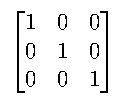
\includegraphics{identity_matrix}
  \caption{\gls*{identity-matrix}的示例:这是
    $\pmb{I}_3$\label{fig:identity_matrix}}
\end{figure}

$\pmb{A}$ 的\gls*{matrix-inversion}表示为 $\pmb{A}^{-1}$,它被定义为这样的矩阵:
\begin{equation}
  \pmb{A}^{-1}\pmb{A} = \pmb{I}_n
  \label{eq:matrix-inverse}
\end{equation}

现在我们可以通过以下步骤解方程~\ref{eq:system_of_linear_equations}:
\begin{align}
  \pmb{A}\pmb{x} &= \pmb{b} \\
  \pmb{A}^{-1}\pmb{A}\pmb{x} &= \pmb{A}^{-1}\pmb{b} \\
  \pmb{I}_n\pmb{x} &= \pmb{A}^{-1}\pmb{b} \\
  \pmb{x} &= \pmb{A}^{-1}\pmb{b}
\end{align}

当然,这依赖于可能找到 $\pmb{A}^{-1}$。我们在接下来一节中讨论 $\pmb{A}^{-1}$ 存在
的条件。

当 $\pmb{A}^{-1}$ 存在时,存在几种不同算法用于在闭合式中找到它。理论上,同样的逆
矩阵可以被用于多次解不同 $\pmb{b}$ 值的方程。然而,$\pmb{A}^{-1}$ 主要作为一个假
设的工具使用,实际上不应该被用在大多数软件应用中。由于在一个数字计算机
中 $\pmb{A}^{-1}$ 可以仅由有限精度表示,利用 $\pmb{b}$ 值的算法通常可以取得更精确
的 $\pmb{x}$ 的估算。

\section{线性相关和生成空间}
\label{sec:linear_dependence_and_span}

为使 $\pmb{A}^{-1}$ 存在,方程~\ref{eq:system_of_linear_equations} 必须对每
个 $\pmb{b}$ 的值有唯一的解。然而,方程系对有些 $\pmb{b}$ 的值也可能无解或有无限
多解。对一个特定的 $\pmb{b}$ 不可能有介于一个和无限多个之间的解;如果 $\pmb{x}$
和 $\pmb{y}$ 都是解,那么
\begin{equation}
  \pmb{z} = \alpha\pmb{x} + (1 - \alpha)\pmb{y}
\end{equation}
对于任意实数 $\alpha$ 也是一个解。

为了分析方程有多少解,我们可以把 $\pmb{A}$ 的列看做指向从\textbf{原点}(由全部
为 $0$ 的向量指定的点)出发的不同方向,并确定有多少路径到达 $\pmb{b}$。在这个观点
下,$\pmb{x}$ 的每个元素指定了我们沿着每个方向要走多远,这里 $x_i$ 指定沿着
列 $i$ 移动多远:
\begin{equation}
  \pmb{A}\pmb{x} = \sum_{i}x_i\pmb{A}_{:,i}
\end{equation}

通常,这种类型的操作被称为\emph{\gls{linear-comb}}。正式地,一个由一
组\gls*{vecs} ${\pmb{v}^{(1)}, \ldots, \pmb{v}^{(i)}}$ 构成的\gls*{linear-comb},
是将每个\gls*{vec} $\pmb{v}^{(i)}$ 乘以一个相应的标量系数并且把结果相加:
\begin{equation}
  \sum_{i}c_i\pmb{v}^{(i)}
\end{equation}

一组向量的\emph{\gls{span}}\,是由原始\gls*{vecs}的\gls*{linear-comb}得到的所有点
的集合。

确定 $\pmb{A}\pmb{x} = \pmb{b}$ 是否有一个解,相当于测试 $\pmb{b}$ 是否
在 $\pmb{A}$ 列中的\gls*{span}。这个特定的\gls*{span}被称
为\emph{\gls{column-space}}\,或者 $\pmb{A}$ 的\emph{\gls{range}}。

为了使方程系 $\pmb{A}\pmb{x} = \pmb{b}$ 对所有 $\pmb{b} \in \mathbb{R}^m$ 的所有
值有唯一解,我们需要 $\pmb{A}$ 的所有\gls*{column-space}为 $\mathbb{R}$。如
果 $\mathbb{R}^m$ 中的任何点被排除于\gls*{column-space}之外,那个点是一个潜在的无
解的 $\pmb{b}$ 值。$\pmb{A}$ 的所有\gls*{column-space}是 $\mathbb{R}^m$ 的需求,
立即暗示了 $\pmb{A}$ 必须有至少 $m$ 个列,即 $n \geq m$。否
则,\gls*{column-space}的维度会小于 $m$。例如,考虑一个 $3 \times 2$ 的矩阵。目
标 $\pmb{b}$ 是 3 维的,但是 $\pmb{x}$ 仅仅是 2 维,所以修改 $\pmb{x}$ 的值最好情
况下允许我们描绘出一个 $\mathbb{R}^3$ 中的 2 维平面。方程当且仅当 $\pmb{b}$ 位于
平面上时有一个解。

对于每个点有一个解,$n \geq m$ 仅仅是一个必要条件。它不是充分条件,因为有可能一些
列是冗余的。考虑一个 $2 \times 2$ 的矩阵,其中两列都是相同的。这与一个仅含有一个
重复列的 $2 \times 1$ 的矩阵 有相同的\gls*{column-space}。换句话说,即使有两
列,\gls*{column-space}仍然仅仅是一条线,无法包含所有的 $\mathbb{R}^2$。

正式地,这种冗余被称为\emph{\gls{linear-dep}}。一个\gls*{vecs}集,如果其中没有一
个\gls*{vec}是其它集和中\gls*{vecs}的\gls*{linear-comb},那么这
个\gls*{vecs}集是\emph{\gls{linearly-indep}}\,的。如果我们往集合中加上一
个\gls*{vec},它是一个集合中其它\gls*{vecs}的\gls*{linear-comb},那么新
的\gls*{vec}并不往集合的\gls*{span}中增加任何点。这意味着对于矩阵
的\gls*{column-space}要包含所有 $\mathbb{R}^m$,这个矩阵必须含有至少一
个 $m$ 个\gls*{linearly-indep}列的集合。这个条件是方
程~\ref{eq:system_of_linear_equations} 的必要条件和充分条件,使得方程对每
个 $\pmb{b}$ 值有一个解。注意这个需求中的集合,是正好
有 $m$ 个\gls*{linear-indep}的列,不是至少 $m$ 列。没有 $m$ 维\gls*{vecs}的集合可
以有多于 $m$ 个互相\gls*{linearly-indep}的列,但是一个具有多于 $m$ 列的矩阵可能有
多于一个这样的集合。

为了使矩阵有一个转置,我们另外需要确保方程~\ref{eq:system_of_linear_equations} 对
每一个 $\pmb{b}$ 的值\textbf{最多}有一个解。为此,我们需要确保矩阵有最多 $m$ 个列。
否则就有多于一个方法来确定每个解的参数。

综合起来,这意味着矩阵必须是\emph{\gls{square}},即,我们需要 $m = n$ 并且所有的
列必须是\gls*{linearly-indep}。一个具有\gls*{linearly-dep}列的方块矩阵被称
为\emph{\gls{singular}}。

如果 $\pmb{A}$ 不是矩阵或者是方块矩阵但不是\gls*{singular},仍然可能解这个方程。
但是我们不能使用\gls*{matrix-inversion}的方法来找出解。

目前为止我们已经讨论过了在左边乘的逆矩阵。也可能定义一个在右边乘的逆:
\begin{equation}
  \pmb{A}\pmb{A}^{-1} = \pmb{I}
\end{equation}

对于方块矩阵,左边求逆和右边求逆是相同的。

\section{范数}
\label{sec:norms}

有时候我们需要测量一个\gls*{vec}的长度。在\gls*{ml}中,我们通常使用一个被称
为\emph{\gls{norm}}\,的函数测量\gls*{vecs}的长度。正式地,对于
$p \in \mathbb{R}, p \geq 1$,$L^p$ 的范数由
\begin{equation}
  \|\pmb{x}\|_p = \left(\sum_i|x_i|^p\right)^{\frac{1}{p}}
\end{equation}
给出。

这些范数,包括 $L^p$ 范数,是将\gls*{vecs}映射为非负值的函数。凭直觉地,一
个\gls*{vec} $\pmb{x}$ 的范数测量从原点到点 $\pmb{x}$ 的距离。更严格地,一个范数
是满足以下特性的任意函数 $f$:
\begin{itemize}
\item $f(\pmb{x}) = 0 \Rightarrow \pmb{x} = \pmb{0}$
\item $f(\pmb{x} + \pmb{y}) \leq f(\pmb{x}) + f(\pmb{y})$
  (\emph{\gls{tri-inequal}}\,)
\item $\forall \alpha \in \mathbb{R}, f(\alpha \pmb{x}) = |\alpha|f(\pmb{x})$
\end{itemize}

具有 $p = 2$ 的 $L^2$ 范数被称为\emph{\gls{eu-norm}}。它是从原点到点 $\pmb{x}$ 的
欧几里德距离。$L^2$ 范数被频繁地使用在\gls*{ml}中以至于它常常被简单表示
为 $\|\pmb{x}\|$,而忽略其下标 $2$。通常也使用平方 $L^2$ 范数测量一个\gls*{vec}的
长度,它可以简单地由 $\pmb{x}^{\top}\pmb{x}$ 来计算。

平方 $L^2$ 范数在数学和计算上比 $L^2$ 范数本身更方便。例如,每个平方 $L^2$ 范数对
于每一个 $\pmb{x}$ 元素的导数,仅依赖于对应的 $\pmb{x}$ 的元素,而所有 $L^2$ 范数
的导数依赖于整个\gls*{vec}。在许多环境中,平方 $L^2$ 范数可能是不受欢迎的,因为它
在原点附近缓慢地增长。在几个\gls*{ml}应用中,区分完全为 $0$ 的元素和很小但非 $0$
的元素是很重要的。在这些情况下,我们转而采用一个在所有位置以相同速率增长,但是在
数学上保留简单特性的函数:$L^1$ 范数。$L^1$ 范数可以简化为:
 \begin{equation}
  \|\pmb{x}\|_1 = \sum_i|x_i|
\end{equation}

当 $0$ 和 非 $0$ 元素非常重要时,$L^1$ 范数被普遍使用在\gls*{ml}中。每次一
个 $\pmb{x}$ 元素从 $0$ 移动了 $\epsilon$,$L^1$ 范数增加了 $\epsilon$。

我们有时候通过计算非 $0$ 元素的个数来测量\gls*{vec}的大小。有些作者把这个函数表示
为``$L^0$''范数,但这是个错误的术语。一个\gls*{vec}中的非 $0$ 元素的个数不是一个
范数,因为通过 $\alpha$ 来调整\gls*{vec}不改变非 $0$ 元素的个数。$L^1$ 模常常被用
作非 $0$ 元素个数的代替者。

另一个在\gls*{ml}中普遍出现的范数是
$L^{\infty}$,也被称为\emph{\gls{max-norm}}。这个范数简化为\gls*{vec}中最大幅度元
素的绝对值,
\begin{equation}
  \|\pmb{x}\|_{\infty} = \max_i|x_i|
\end{equation}

有时候我们也想要测量矩阵的大小。在\gls*{dl}的环境中,最普遍的方式是以不同的、费解
的\emph{\gls{fr-norm}}
\begin{equation}
  \|A\|_F = \sqrt{\sum_{i,j}A_{i,j}^2}
\end{equation}
它类似于一个\gls*{vec}的 $L^2$ 范数。

两个\gls*{vecs}的点乘可以重写为范数的形式。具体来说,
\begin{equation}
  \pmb{x}^{\top}\pmb{y} = \|\pmb{x}\|_2\|\pmb{y}\|_2\cos \theta
\end{equation}
其中 $\theta$ 是 $\pmb{x}$ 和 $\pmb{y}$ 之间的夹角。

\section{特殊类型的矩阵和向量}
\label{sec:special_kinds_of_matrices_and_vectors}

一些特别有用的特殊类型的矩阵和\gls*{vecs}。

\emph{\gls{diag}}\,矩阵大部分由 $0$ 组成,仅仅沿着主对角线有非 $0$ 元素。正式地,
一个矩阵 $\pmb{D}$ 当且仅当对所有 $i \neq j$ 的 $D_{i,j} = 0$ 时是对角线的。我们
已经见过了一个对角矩阵的例子:单位矩阵,其中所有的对角线元素为 $1$。我们写
成 $\mathrm{diag}(\pmb{v})$ 来表示一个方块对角矩阵,其中对角线元素由\gls*{vec}
$\pmb{v}$ 的元素给出。对角矩阵在某种程度上让人感兴趣是因为被一个对角矩阵相乘,在
计算上是非常有效率的。计算 $\mathrm{diag}(\pmb{v})\,\pmb{x}$,我们只需要用 $v_i$
来调整每个元素
$x_i$。换句话说,$\mathrm{diag}(\pmb{v})\,\pmb{x} = \pmb{v} \odot \pmb{x}$。对一
个方块对角矩阵求逆也同样高效。仅当每个对角线元素为非 $0$ 时矩阵的逆存在,在这种情
况下,$\mathrm{diag}(\pmb{v})^{-1} = \mathrm{diag}([1/v_1, \ldots,
1/v_n]^{\top})$。在许多情况下,我们可能会得到一些非常一般的以任意矩阵形式
的\gls*{ml}算法,但通过限制一些矩阵为对角矩阵可获得一个代价更低的(和更少描述性的)
算法。

不是所有的对角矩阵需要是方块型的。构建一个矩形的对角矩阵是可能的。非方块对角矩阵
没有逆,但是它仍然可能被它们以较低的代价相乘。对于一个非方块对角矩阵 $\pmb{D}$,
乘积 $\pmb{D}\pmb{x}$ 会涉及到调整 $\pmb{x}$ 的每个元素,并且,如果 $\pmb{D}$ 的
高度比宽度大则往结果中连接一些 $0$,或者当 $\pmb{D}$ 的宽度大于高度时则舍
弃\gls*{vec}的最后一些元素。

一个\emph{\gls{symmetric}}\,矩阵常常出现在其中的元素由一些有两个参数的函数生成的
时候,其元素不依赖于这两个参数的顺序。例如,如果 $\pmb{A}$ 是一个距离测量的矩
阵,$\pmb{A}_{i,j}$ 给出了从点 $i$ 到点 $j$ 的距离,那么因为距离函数是对称
的,$\pmb{A}_{i,j} = \pmb{A}_{j,i}$。

一个\emph{\gls{unit-vec}}\,是一个具有\emph{\gls{unit-norm}}\,的\gls*{vec}:
\begin{equation}
  \|\pmb{x}\|_2 = 1
\end{equation}

一个\gls*{vec} $\pmb{x}$ 和一个 \gls*{vec} $\pmb{y}$,如
果 $\pmb{x}^{\top}\pmb{y} = 0$,那么它们是相互\emph{\gls{ortho}}。如果两
个\gls*{vecs}都有非 $0$ \gls*{norm},这意味着它们以 $90^{\circ}$ 角相互垂直。
在 $\mathbb{R}^n$ 中,最多有 $n$ 个具有非 $0$ \gls*{norm}的\gls*{vecs}可以相互正
交。如果\gls*{vecs}不仅是正交的,还有\gls*{unit-norm},那么我们称它们
是\emph{\gls{orthonormal}}。

一个\emph{\gls{orthonormal-matrix}}\,是一个方块矩阵,其各行是相
互\gls*{orthonormal},而各列也是相互\gls*{orthonormal}:
\begin{equation}
  \pmb{A}^{\top}\pmb{A} = \pmb{A}\pmb{A}^{\top} = \pmb{I}
\end{equation}

这表示
\begin{equation}
  \pmb{A}^{-1} = \pmb{A}^{\top}
\end{equation}
所以正交矩阵有趣在它们的逆可以以很低的代价来计算。认真注意正交矩阵的定义。相反,
它们的行不仅仅是正交的,而且是完全标准正交的。没有一个特殊的术语来定义一个行或列
正交但不是标准正交的矩阵。

\section{特征分解}
\label{sec:eigendecomposition}


\chapter{Probability and Information Theory}
\label{ch:prob}

\chapter{数值计算}
\label{ch:numerical}

\chapter{机器学习基础}
\label{ch:ml}

\part{深度学习:现代实践}
\label{part_practical}

\chapter{深度前驱网络}
\label{ch:mlp}

\chapter{深度学习的规范化技术}
\label{ch:regularization}

\chapter{训练深层模型的优化技术}
\label{ch:optimization}

\chapter{Convolutional Networks}
\label{ch:convnets}

\chapter{序列建模:循环和递归网络}
\label{ch:rnn}

\chapter{Practical methodology}
\label{ch:guidelines}

\chapter{Applications}
\label{ch:applications}

\part{深度学习研究}
\label{part_research}

本书此部分介绍了当前深度学习研究社区中有关深度学习更深的愿景及更加高级的方法. \\

在本书前面的章节中,我们已经展示了如何去解决监督学习问题——在给定足够的映射样本的情况下,如何学习将一个向量映射到另一个向量. \\

不是所有我们想要解决的问题都是落在这个类别中的. 我们可能希望去产生新的样本,或者确定某些点是新的样本,或者处理遗漏值利用大量的无标记样本或者相关的任务的样本. 当前工业应用的最新发展的不足是我们的学习算法需要大量监督数据来达到足够的精确度. 在这个部分,我们会讨论一些降低对已有模型必要的标记数据量和能够应用在多个任务上的尝试性工作. 达成这些目标通常需要某种形式的无监督学习和半监督学习.\\

很多深度学习算法都是被设计成解决无监督学习问题的,但是相比深度学习在监督学习问题上已经取得的处处开花的成就,没有一个真正解决好这个问题. 本书此部分,我们给出已有的无监督学习方法和一些热门的有关如何在此领域取得进展的思考.\\

无监督学习的困难之处在于需要建模的随机变量的维度太高. 这会导致两个不同的挑战:统计学挑战和计算挑战. \emph{统计学挑战}说的是泛化:我们需要的能够区分类别的配置的数量会与有意义的维度的数量呈指数级增长,并且这数字很快超过我们可能拥有的样本数量(或者受到计算资源的限制). 而 \emph{计算挑战}则是和高维分布相关,很多算法学习或者使用一个训练好的模型(特别是基于估计一个显式的概率函数)会引入与维度呈指数级增长的难解的计算量.\\

有了概率模型,计算挑战是来自进行难解推断或者就是规范化分布的需求.\\

\begin{enumerate}
\item \textbf{难解推断}:推断主要会放在第 \ref{ch:inference} 章讨论. 推断就是包含了在一个刻画了变量 $a$,$b$ 和 $c$ 联合分布的模型下,给定另外的变量 $b$,猜测某些变量 $a$ 可能的值的问题. 为了计算这种条件概率,我们需要对变量 $c$ 的可能值进行求和并且计算一个对 $a$ 和 $c$ 的值求和的规范化常量.
\item \textbf{难解规范化化常量(配分函数)}:这部分会在第 \ref{ch:partition} 章进行讨论. 规范化概率函数的常量在推断和学习中均会出现. 不幸的是,学习这样的模型通常需要计算配分函数关于模型参数的梯度. 这种计算通常和计算配分函数本身一样难解. 蒙特卡洛马尔科夫链(Monte Carlo Markov Chain,后简称 MCMC)方法(见第 \ref{ch:monte_carlo} 章)通常用来解决配分函数问题(计算本身或者其梯度). 然而,MCMC 方法当模型分布的\gls*{mode}很多且分隔明显,特别是高维空间中时就遇到了麻烦(17.5 节).
\end{enumerate}

一种处理这些难解计算问题的方法就是近似,很多近似方法在本书这个部分进行讨论. 另一个这里也会介绍的有趣方法就是通过设计来避免这些难解计算,这些方法就是非常有意义的. 近几年几种生成式模型已经被研究者提出来了,出发点就是良好的设计避免难解计算. 目前生成式模型的研究方法的几种变化在第 \ref{ch:generative_models} 章讨论. \\

第 \ref{part_research} 部分 对那些想要理解深度学习领域已有的观点的宽广,并且志在推进真正的人工智能领域的发展的研究者来说最为重要. 


\chapter{线性因子模型}
\label{ch:linear_factors}

\chapter{Autoencoders}
\label{ch:autoencoders}

\chapter{表示学习}
\label{ch:representation}

\chapter{深度学习的结构化概率模型}
\label{ch:graphical_models}

\chapter{Monte Carlo Methods}
\label{ch:monte_carlo}

\chapter{处理配分函数}
\label{ch:partition}

在 16.2.2 节,我们看到了很多概率模型(通常是无向图模型)是由一个没有正规化的概率分布 $\tilde{p}(\mathbf{x};\theta)$ 定义的. 我们必须通过除以一个配分函数 $Z(\pmb{\theta})$ 来正规化 $\tilde{p}$ 才能得到一个合法的概率分布:

\begin{equation}  \label{eq:pyth}
p(\mathbf{x};\pmb{\theta}) = \frac{1}{Z(\pmb{\theta})} \tilde{p}(\mathbf{x}; \pmb{\theta}).
\end{equation}

配分函数对连续型变量是积分,而对离散型变量是对所有状态的非正规化概率进行求和:

\begin{equation}  \label{eq:pyth}
\int \!\tilde{p}(\pmb{x})\, \mathrm{d}\pmb{x}
\end{equation}

或者

\begin{equation}  \label{eq:pyth}
\sum_{x} \tilde{p}(\pmb{x}).
\end{equation}

这个操作对很多有趣的模型都是难解的. 

如我们将在第 20 章中看到的,有些深度学习模型被设计成有可解的正规化常量,或者被设计成不需要包含计算 $p(\mathbf{x})$ 的. 然而,其他的模型需要直接面对难解的配分函数的挑战. 本章,我们会给出一些用来训练和评估那些有着难解配分函数的模型的技术. 

\section{对数似然梯度 log-likelihood gradient}
\label{sec:llg}

让通过最大似然估计在学习无向的模型中尤其困难的原因是配分函数依赖于参数. 对数似然函数关于参数的梯度包含一个配分函数的梯度项:

\begin{equation}  \label{eq:pyth}
\nabla_{\pmb{\theta}} \log p(\mathbf{x};\pmb{\theta}) = \nabla_{\pmb{\theta}} \log \tilde{p}(\mathbf{x};\pmb{\theta}) - \nabla_{\pmb{\theta}} \log Z\pmb{\theta})
\end{equation}

这是一个著名的分解——将学习分成正负两个部分.\\

对大多数有趣的无向图模型,负部(negative phase)是困难的. 没有隐含变量或者隐含变量间的交互很少的模型通常会有可解的正部(positive phase) 典型的包含一个直接简单的正部而非常困难的负部的模型是 RBM,它的隐含单元在给定可见单元的时候是彼此是条件独立的. 而正部困难的例子是,隐含元之间的交互特别复杂,这个在第 19 章会讲述. 本章聚焦在负部的难解性上.\\

让我们仔细看看 $\log Z$ 的梯度:

\begin{equation}  \label{eq:pyth}
\frac{\partial}{\partial \pmb{\theta}} \log Z
\end{equation}
\begin{equation}  \label{eq:pyth}
=\frac{\frac{\partial}{\partial \pmb{\theta}} Z}{Z}
\end{equation}
\begin{equation}  \label{eq:pyth}
=\frac{\frac{\partial}{\partial \pmb{\theta}} \sum_{\mathbf{x} \tilde{p}(\mathbf{x})}}{Z}
\end{equation}
\begin{equation}  \label{eq:pyth}
=\frac{\sum_{\mathbf{x} \frac{\partial}{\partial \pmb{\theta}} \tilde{p}(\mathbf{x})}}{Z}
\end{equation}

对于那些对所有的 $\mathbf{x}$ 保证 $p(\mathbf{x}) > 0$ 的模型,我们可以为 $\tilde{p}(\mathbf{x})$ 替换 $\exp(\log \tilde{p}(\mathbf{x})$:
\begin{equation}  \label{eq:pyth}
\frac{\sum_{\mathbf{x} \frac{\partial}{\partial \pmb{\theta}} \exp(\log \tilde{p}(\mathbf{x}))}}{Z}
\end{equation}
\begin{equation}  \label{eq:pyth}
=\frac{\sum_{\mathbf{x} \exp(\log\tilde{p}(\mathbf{x})) \frac{\partial}{\partial \pmb{\theta}} \tilde{p}(\mathbf{x})}}{Z}
\end{equation}
\begin{equation}  \label{eq:pyth}
=\frac{\sum_{\mathbf{x} \tilde{p}(\mathbf{x}) \frac{\partial}{\partial \pmb{\theta}} \tilde{p}(\mathbf{x})}}{Z}
\end{equation}
\begin{equation}  \label{eq:pyth}
=\sum_{x}p(\mathbf{x}) \frac{\partial}{\partial \pmb{\theta}} \log \tilde{p}(\mathbf{x})
\end{equation}
\begin{equation}  \label{eq:pyth}
=\mathbf{E}_{x\sim p(\mathbf{x})} \frac{\partial}{\partial \pmb{\theta}} \tilde{p}(\mathbf{x}).
\end{equation}

这个推导对离散的 $\pmb{x}$ 进行求和,类似地也可以对连续的 $\pmb{x}$ 进行积分. 在连续版本的推到中,我们使用 Leibniz 法则在积分符号下进行微分,获得等式:
\begin{equation}  \label{eq:pyth}
\frac{\partial}{\partial \pmb{\theta}} \int \!\tilde{p}(\mathbf{x}) \, \mathrm{d}\pmb{x} = \int \!\frac{\partial}{\partial \pmb{\theta}} \tilde{p}(\pmb{x}) \,\mathrm{d}\pmb{x}.
\end{equation}

等式只有在 $\tilde{p}$ 和 $\frac{\partial}{\partial \pmb{\theta}} \tilde{p}(\mathbf{x})$ 满足某种规范化条件时可用. 用测度论的术语,条件是:
\begin{enumerate*}[label={\roman*)}]
\item $\tilde{p}$ 必须是一个对每个 $\pmb{\theta}$ 值的 $\pmb{x}$ 的 Lebesgue-可积函数;
\item $\frac{\partial}{\partial \pmb{\theta}} \tilde{p}(\mathbf{x})$ 必须对所有的 $\pmb{\theta}$ 和几乎所有的 $\pmb{x}$ 存在
\item 必须存在一个可积分函数 $R(\pmb{x})$ 控制住 $\frac{\partial}{\partial \pmb{\theta}} \tilde{p}(\mathbf{x})$(如对所有的 $\pmb{\theta}$ 和几乎所有的 $\pmb{x}$ 有 $|\frac{\partial}{\partial \pmb{\theta}}\tilde{p}(\mathbf{x})|\leq R(\pmb{x})$).
\end{enumerate*}

幸运的是,大多数机器学习模型满足这些条件.\\

这个等式
\begin{equation}  \label{eq:pyth15}
\nabla_{\pmb{\theta}} \log Z = \mathbb{E}_{\mathbf{x}\sim p(\mathbf{x})} \nabla_{\pmb{\theta}} \log \tilde{p}(\mathbf{x})
\end{equation}
是一系列 Monte Carlo 方法的基础,可以用来近似最大化那些有着难解的配分函数的模型的似然函数.\\

学习无向模型的 Monte Carlo 方法给出了一个直觉框架,我们可以利用这样的框架来思考正部和负部. 在正部中,我们对那些从数据抽取的 $\pmb{x}$ 增加 $\log \tilde{p}(\mathbf{x})$. 在负部中,我们通过减少从模型分布中个采样的 $\log \tilde{p}(\mathbf{x})$ 来降低配分函数.\\

在深度学习文献中,通常会用能量函数参数化 $\log \tilde{p}$(Eq. 16.7). 在这种情况下,我们可以将正部解释为降低训练样本的能量,而负部则是提升从模型中采样的样本的能量,如图 18.1 所示.

\section{随机最大似然和对比散度}

实现 \eqref{eq:pyth15} 的基本方式是每次需要计算梯度时从一个随机初始化状态的 Markov 链的集合中进行老化(burning). 在使用随机梯度下降算法进行学习时,这个 Markov 链必须每个梯度步都已经老化. 这个想法就是算法~\ref{alg:mcmc}
中的训练过程. 内循环中的 Markov 链老化的计算代价让这个过程在计算上不可行,但是这个过程本身是其他实效的近似算法的起点. 

% \begin{algorithm}[H]
%     设置 $\epsilon$,一个很小的正数作为步长.
%     设置 $\k$,Gibbs 步数,足够长满足老化条件. 在一个小的图像块(image patch)上训练 RBM 可能需要 $100$.


%   \caption{用来最大化对数似然函数的 MCMC 算法,使用梯度下降来处理难解的配分函数}
%   \label{alg:algorithm1}
% \end{algorithm}

\begin{algorithm}
\begin{algorithmic}
\caption{用来最大化对数似然函数的 MCMC 算法,使用梯度下降来处理难解的配分函数}
\label{alg:mcmc}
\STATE 设置 $\epsilon$,一个很小的正数作为步长.
\STATE 设置 $k$,Gibbs 步数,足够长满足老化条件. 在一个小的图像块(image patch)上训练 RBM 可能需要 $100$.
\WHILE{未收敛}
	\STATE 从训练集中采样 $m$ 个样本 $\{x^{(1)},\dots,x^{(m)}\}$ 的一个\gls{minibatch}.
	\STATE $\mathbf{g} \leftarrow \frac{1}{m}\,\sum_{i = 1}^{m} \nabla_{\pmb{\theta}} \log\tilde{p}(x^{(i)};\pmb{\theta})$.
	\STATE 将随机值为对应 $m$ 个样本 $\{\tilde{\mathbf{x}}^{(1)},\dots,\tilde{\mathbf{x}}^{(m)}\}$ 初始化(如,从一个均匀分布或者正态分布,或者也可能是有匹配于模型边缘分布的分布).
	\FOR{$i = 1$ to $k$}
	 	\FOR{$j = 1$ to $m$}
		\STATE $\tilde{\mathbf{x}}^{(j)} \leftarrow \mathrm{gibbs\_update}(\tilde{\mathbf{x}}^{(j)})$
		\ENDFOR
	\ENDFOR
	\STATE $\mathbf{g} \leftarrow \frac{1}{m}\,\sum_{i = 1}^{m} \nabla_{\pmb{\theta}} \log\tilde{p}(x^{(i)};\pmb{\theta})$.
	\STATE $\pmb{\theta} \leftarrow \pmb{\theta} + \epsilon \mathbf{g}$.
\ENDWHILE

\end{algorithmic}
\end{algorithm}

我们可以将最大似然 MCMC 方法看成是尝试达到两个力量的平衡,一个力量在数据出现时将模型分布上推,而另一个则在模型的样本出现时下推模型分布. 
图~\ref{fig:18.1}

% \begin{figure}
% \centering 
% 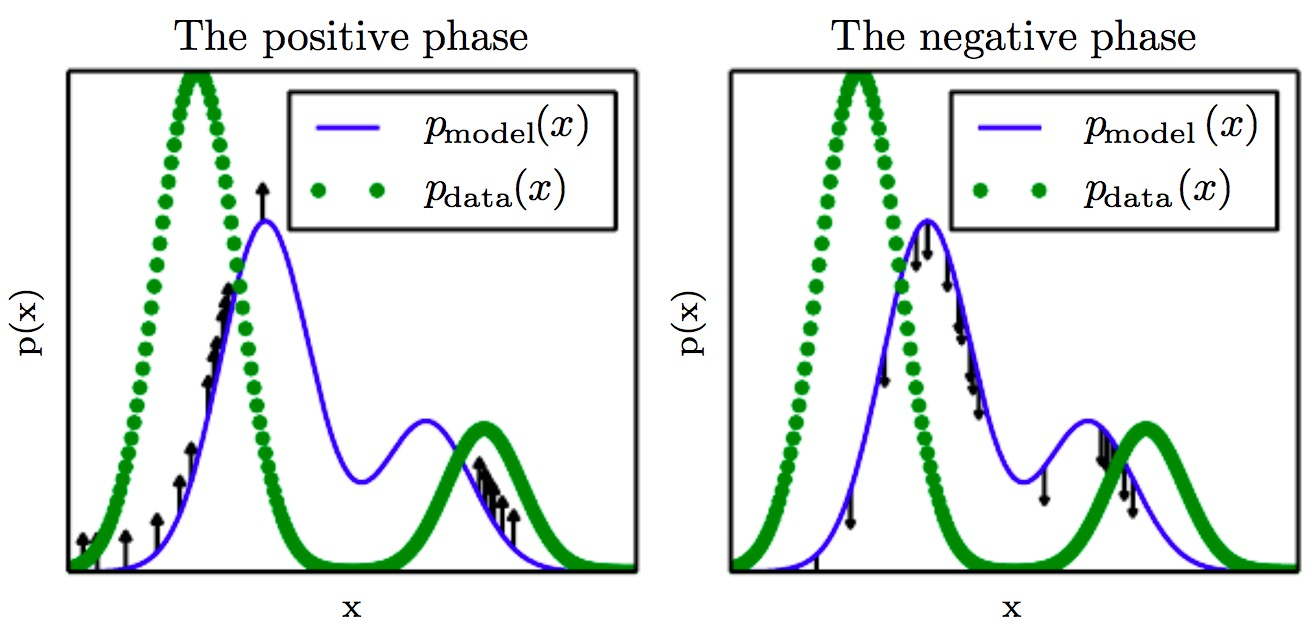
\includegraphics[width=1.0\textwidth]{figure18-1} 
% \caption{算法~\ref{alg:mcmc} 的正部和负部. 左图,在正部中,我们从数据分布中采样,上推他们的未规范化概率. 可能在数据中的点被更多地上推. 右图,在负部中,我们从模型的概率分布采样,下推他们的未规范化概率. 这样会抵制正部的倾向于在每个处都给未规范化概率加上一个大的常量. 当数据分布和模型分布等同时,正部和负部分别有同样的机会上推和下推. 这种情形出现时,就不再回产生梯度(期望形式),训练必须终止.}
% \label{fig:18.1} 
% \end{figure}

\begin{figure}[htp]
\centering 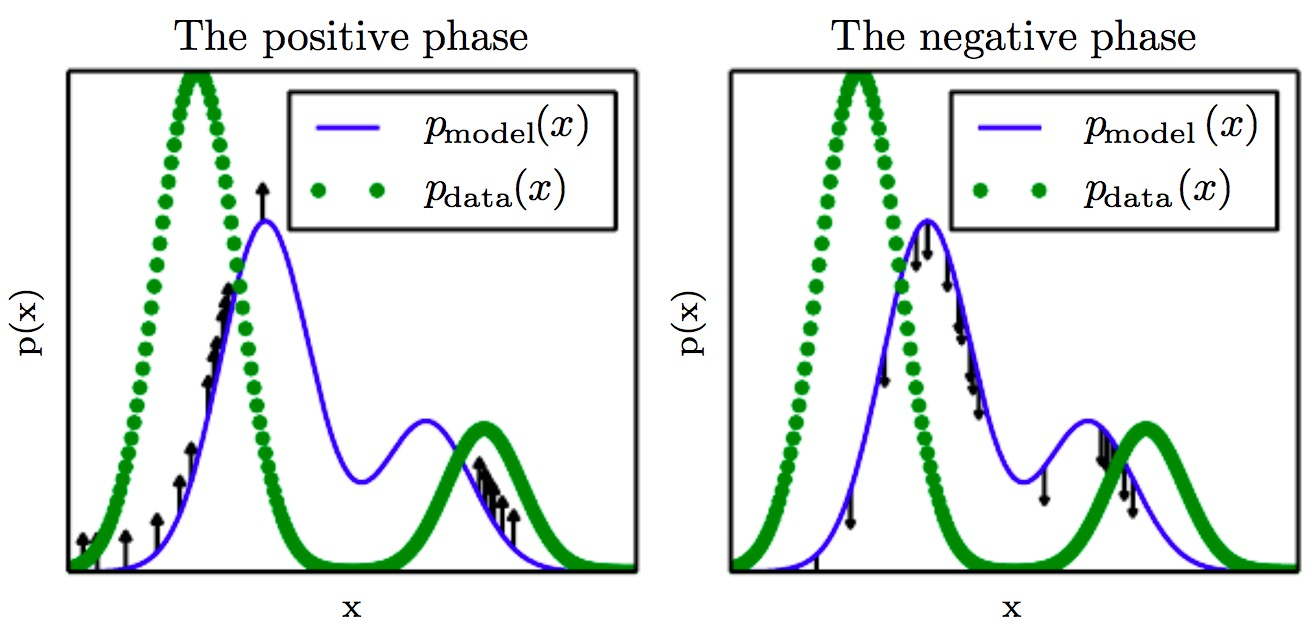
\includegraphics[width=1.0\textwidth]{figure18-1} 
\caption{算法~\ref{alg:mcmc} 的正部和负部. 左图,在正部中,我们从数据分布中采样,上推他们的未规范化概率. 可能在数据中的点被更多地上推. 右图,在负部中,我们从模型的概率分布采样,下推他们的未规范化概率. 这样会抵制正部的倾向于在每个处都给未规范化概率加上一个大的常量. 当数据分布和模型分布等同时,正部和负部分别有同样的机会上推和下推. 这种情形出现时,就不再回产生梯度(期望形式),训练必须终止.} 
\label{fig:18.1}
\end{figure}




\chapter{近似推断}
\label{ch:inference}

\chapter{Deep Generative Models}
\label{ch:generative_models}


% \appendix
% appendix chapters here

\backmatter{}

\bookmarksetup{startatroot}

\printbibliography[
	heading=bibintoc,
	title={参考文献}
]
\printindex
\printglossary[title={术语表}]

\end{document}
